\documentclass{beamer}

%
% Escolha o formato da  sua Apresentação 
%
% Para mais temas, esquemas de cores e fontes, veja:
% http://deic.uab.es/~iblanes/beamer_gallery/index_by_theme.html
% (link em Inglês)
%

\mode<presentation>
{
  \usetheme{Warsaw}       
  % escolha do tema, experimente Darmstadt, Madrid, Dresden, ...
  \usecolortheme{default} 
  % escolha do esquema de cor, experimente albatross, beaver, crane, ...
  \usefonttheme{default}  
  % escolha da fontes, experimente serif, structurebold, ...
  \setbeamertemplate{navigation symbols}{}
  \setbeamertemplate{caption}[numbered]
} 

\usepackage[brazil]{babel}
\usepackage[T1]{fontenc}
\usepackage[utf8]{inputenc}

\title{Revolução dos Cravos}
\author{Otelo Saraiva de Carvalho}
\institute{Portugal}
\date{25 de Abril 1975}

\begin{document}

\begin{frame}
  \titlepage
\end{frame}



\begin{frame}{Indíce}
  \tableofcontents
\end{frame}

\section{Agenda}

\begin{frame}{Agenda}

\begin{itemize}
  \item Preparação do Golpe 
  \item Movimentações Militares
  \item Restaurar o Governo
\end{itemize}

\end{frame}

\begin{frame}{Fora da Agenda!}

\begin{itemize}[<+->]
  \item Assalto ao Castelo
  \item Violência nas Ruas
  \item Dispersão de Manifestantes
\end{itemize}

\end{frame}

\section{Revisão}

\begin{frame}{Objectivos principais \& Fatores de Sucesso}

\begin{itemize}
\item O que faz uma nação única:
  \begin{itemize}
    \item Liberdade
    \item Todos os Homens são iguais
  \end{itemize}
\end{itemize}

\begin{block}{Visão comum}
\begin{itemize}
\item Restauro da Liberdade.
\item Um governo para/pelo o povo.
\end{itemize}
\end{block}

\end{frame}

\begin{frame}{Resultados}

\begin{figure}
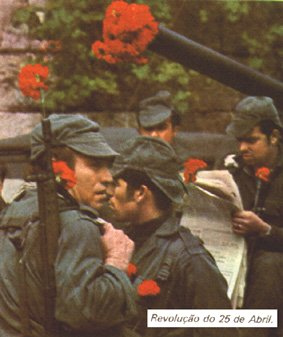
\includegraphics[width=0.3\textwidth]{Cravos.jpg}
\end{figure}

\begin{block}{Número de Mortes}
\begin{equation}
(4 \times 20 - 73) = 7
\end{equation}
\end{block}

\end{frame}

\section{Sumário}

\begin{frame}{Sumário}

\begin{columns}
\begin{column}{0.6\textwidth}
\begin{itemize}
\item Revolução Pacífica
\item Implantação da República
\item Fim da Guerra Colonial
\end{itemize}
\end{column}
\begin{column}{0.4\textwidth}
\begin{itemize}
\item Liberdade
\item União
\item Fraternidade
\end{itemize}
\end{column}
\end{columns}

\end{frame}

\end{document}